\chapter{Ejemplos del lenguaje de marcado \LaTeX{}}

\section{Algunos ejemplos básicos de uso de \LaTeX{}}

  \textbf{Texto} en el párrafo 1.

  \textit{Texto} en el párrafo 2.

  \texttt{Texto} en el párrafo 3.


  \begin{itemize}
  \item Consideración 1
  \item Consideración 2
  \end{itemize}

  % Espacio vertical
  \vspace{0.5cm}
  
  \begin{enumerate}
  \item Punto 1
  \item Punto 2
  \end{enumerate}
  
A continuación se muestra una ecuación:

  \[ \int_{0}^{1}\frac{1}{x^2+1} dx \]

  \section{Figuras y subfiguras}

  Podemos incluir imágenes en formato: png, pdf o jpg.

  En la Figura~\ref{fig:diagrama} se muestra un diagrama\footnote{Realizado con \href{yed}{https://www.yworks.com/products/yed}}, mientras que la Figura~\ref{fig:diagramas} muestra varios diagramas en mosaico, de manera que puedo referirme al segundo diagrama como Figura~\ref{fig:diagrama-2}.

  \begin{figure}[!htb]
    \centering
    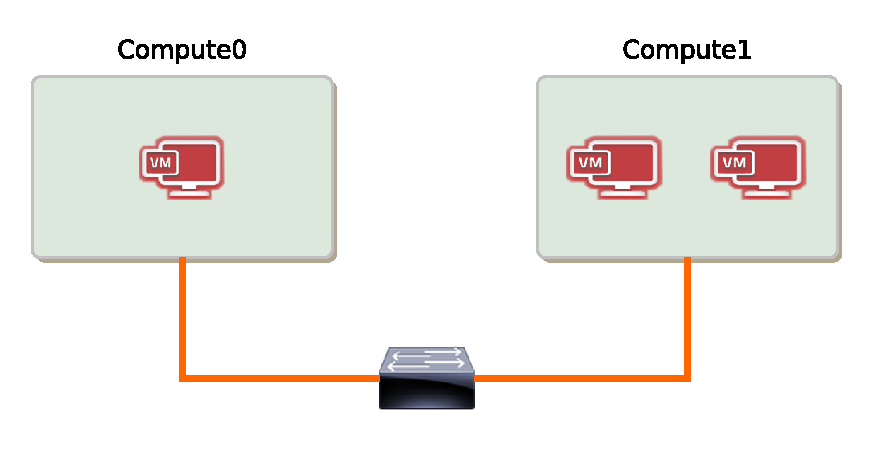
\includegraphics[width=0.8\textwidth]{diagrama.pdf}
    \caption{Esta es una figura que latex decide donde colocar (floating) en el documento.}
    \label{fig:diagrama}
  \end{figure}

  \begin{figure}[h!t]
    \centering
    \begin{subfigure}{0.45\textwidth}
        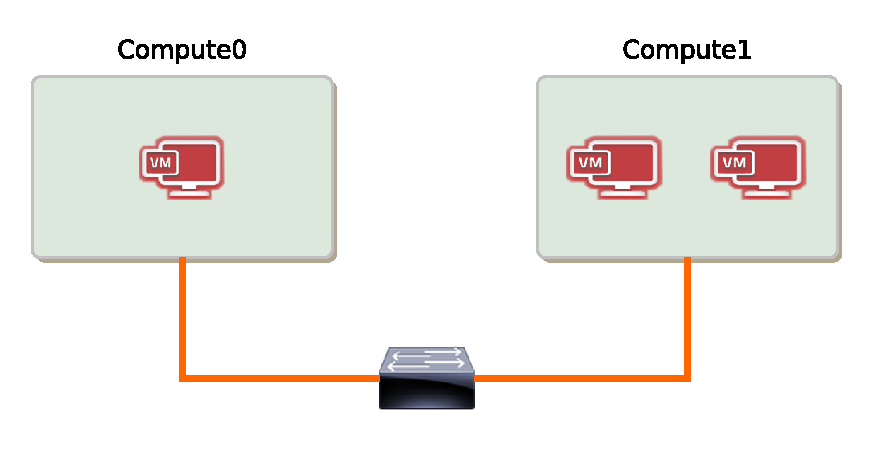
\includegraphics[width=\textwidth]{diagrama.pdf}
        \caption{Copia 1}\label{fig:diagrama-1}
    \end{subfigure}
    \hfill
    \begin{subfigure}{0.45\textwidth}
        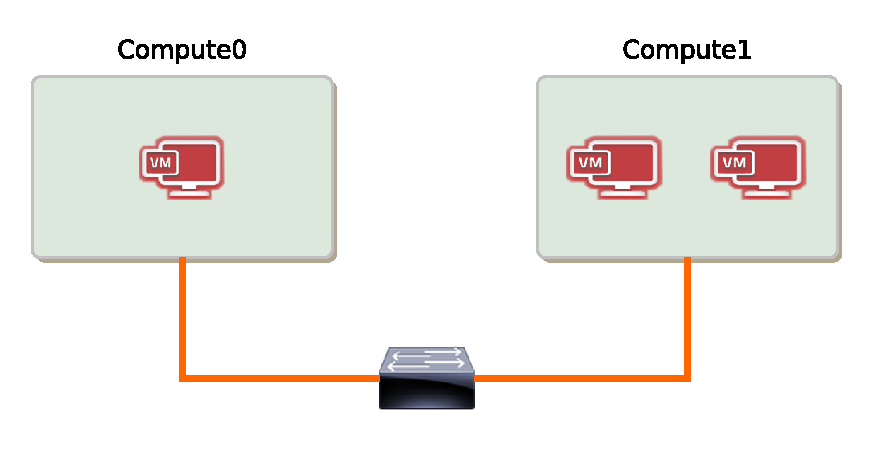
\includegraphics[width=\textwidth]{diagrama.pdf}
        \caption{Copia 2}\label{fig:diagrama-2}
    \end{subfigure}
    \vskip\baselineskip
    \begin{subfigure}{0.45\textwidth}
        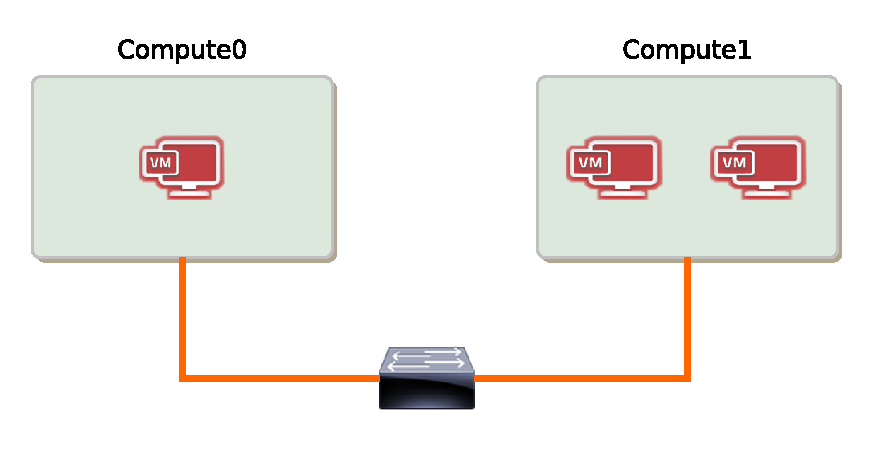
\includegraphics[width=\textwidth]{diagrama.pdf}
        \caption{Copia 3}\label{fig:diagrama-3}
    \end{subfigure}
    \hfill
    \begin{subfigure}{0.45\textwidth}
        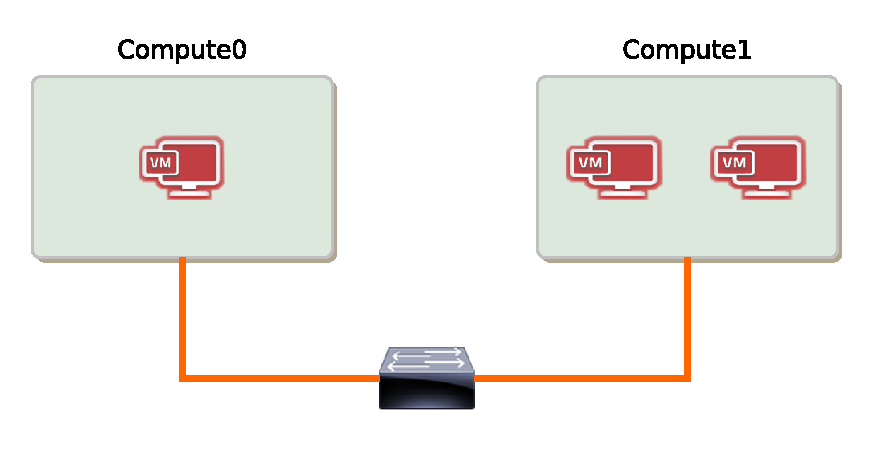
\includegraphics[width=\textwidth]{diagrama.pdf}
        \caption{Copia 4}\label{fig:diagrama-4}
    \end{subfigure}
    \caption{Los cuatro diagramas en mosaico}
    \label{fig:diagramas}
\end{figure}

\section{Tablas}
  
  La Tabla \ref{tab:ejemplo-1} es un ejemplo de una tabla.
  
  \begin{table}[!htb]
    \centering
  \begin{tabular}{|l|c|}
    \hline
    Columna 1 & Columna 2 \\ \hline
    1 & 2 \\ \hline
  \end{tabular}
  \caption{Ejemplo de tabla 1}
  \label{tab:ejemplo-1}
\end{table}

  Existen también tablas más complejas que requieren un mayor control de la posición de los elementos, como la Tabla \ref{tbl:phd-raul} que ha sido extraída de \cite{rpo:tesis-2013}, o de varias páginas, como la Tabla~\ref{tab:long}. 

  \begin{sidewaystable}
    \centering
    \begin{tabular}{|l|c|c|c|c|c||c|c|c||c|c|c|c|c|c|c|c|c|c|}
    \cline{2-17}
    \cline{2-17}
    \multicolumn{1}{l|}{} & \multicolumn{5}{c||}{GROUP I} & \multicolumn{3}{c||}{GROUP II} &
    \multicolumn{8}{c|}{GROUP III}\\
    \cline{2-17}
    \hline
    
    \backslashbox[60mm]{FEATU./CAPAB.}{GENERATOR}
    &
    % Benchmarks
    \begin{sideways}WebStone\end{sideways}&
    \begin{sideways}SPECweb\end{sideways} &
    \begin{sideways}SURGE\end{sideways} &
    \begin{sideways}Web Polygraph\end{sideways} &
    \begin{sideways}TPC-W\end{sideways} &
    
    % Grupo de generadores de carga que producen dinamismo
    \begin{sideways}LoadRunner\end{sideways} &
    \begin{sideways}WebLOAD\end{sideways} &
    \begin{sideways}JMeter\end{sideways} &
          
    % Herramientas para la generación de carga
    \begin{sideways}S-Clients\end{sideways} &
    \begin{sideways}WebJamma\end{sideways} &
    \begin{sideways}Deluge\end{sideways} &
    \begin{sideways}HAMMERHEAD 2\hspace{0.25cm} \end{sideways} &
    \begin{sideways}PTester\end{sideways} &
    \begin{sideways}Siege\end{sideways} &
    \begin{sideways}HTTPERF \end{sideways} &
    \begin{sideways}Autobench\end{sideways}\\
    
    \hline\color{black}\scriptsize{Analytical-Based
    Architecture}& {\color{gray}\faStar{}} & {\color{gray}\faStar{}} &
    {\color{gray}\faStar{}} & {\color{gray}\faStar{}} & {\color{gray}\faStar{}} & {\color{gray}\faStarHalf*{}}& {\color{gray}\faStarHalf*{}}& {\color{gray}\faStarHalf*{}}& & & & &
    & & & \\
    
    \hline\scriptsize{Distributed Architecture}& {\color{gray}\faStar{}} &
    {\color{gray}\faStar{}} & {\color{gray}\faStar{}} &  {\color{gray}\faStar{}} & & {\color{gray}\faStar{}} & {\color{gray}\faStar{}} &  &  &  &  &  &  &
     &  & \\
    
    \hline\scriptsize{Business-Based Architecture} & & {\color{gray}\faStarHalf*{}} & & {\color{gray}\faStarHalf*{}} & {\color{gray}\faStar{}} & {\color{gray}\faStar{}} & {\color{gray}\faStar{}} & {\color{gray}\faStar{}} & & & & & & & & \\
    
    \hline\scriptsize{Client Parameterization} & {\color{gray}\faStar{}} &
    {\color{gray}\faStar{}} & & {\color{gray}\faStarHalf*{}} & {\color{gray}\faStar{}} & {\color{gray}\faStar{}} & {\color{gray}\faStar{}} & {\color{gray}\faStar{}} & & {\color{gray}\faStar{}} & & {\color{gray}\faStarHalf*{}} & & & {\color{gray}\faStarHalf*{}} &  \\
    
    \hline\scriptsize{Workload Types} & & {\color{gray}\faStar{}} & & & {\color{gray}\faStar{}} & {\color{gray}\faStar{}} &{\color{gray}\faStar{}}  & {\color{gray}\faStarHalf*{}}
    & & & & & & & & \\
    
    \hline\scriptsize{Functional Testing} & & & & & & {\color{gray}\faStar{}} &{\color{gray}\faStar{}} &  {\color{gray}\faStarHalf*{}} & & & &{\color{gray}\faStarHalf*{}} &{\color{gray}\faStarHalf*{}}
     &{\color{gray}\faStarHalf*{}} & & {\color{gray}\faStarHalf*{}}\\
    
    \hline\scriptsize{LAN and WAN}& & & & & & & & & {\color{gray}\faStar{}} & & &
    & & & & \\
    
    \hline\scriptsize{Multi-platform}&{\color{gray}\faStar{}}&{\color{gray}
    \faStar{}}&{\color{gray}\faStar{}}&{\color{gray}\faStar{}}&{
    \color{gray}\faStar{}}&{\color{gray}\faStar{}}&{\color{gray}\faStar{}}&{\color{gray}\faStar{}}&{\color{gray}\faStar{}}&{\color{gray}\faStar{}}&{\color{gray}\faStar{}}&{\color{gray}\faStarHalf*{}}&{\color{gray}\faStar{}}&{\color{gray}\faStarHalf*{}}&{\color{gray}\faStar{}}&{\color{gray}\faStar{}}\\
    
    \hline\scriptsize{Ease of Use}& & & & & &{\color{gray}\faStar{}} &{\color{gray}\faStar{}} & {\color{gray}\faStarHalf*{}} & & & & & & & &\\
    
    \hline\scriptsize{Performance Reports} &  
    {\color{gray}\faStarHalf*{}}& 
    {\color{gray}\faStar{}}&&
    {\color{gray}\faStar{}}&
    {\color{gray}\faStar{}}&
    {\color{gray}\faStar{}}&
    {\color{gray}\faStar{}}&
    {\color{gray}\faStar{}}&&&
    {\color{gray}\faStarHalf*{}}&
    {\color{gray}\faStarHalf*{}}&
    {\color{gray}\faStarHalf*{}}&
    {\color{gray}\faStarHalf*{}}&
    {\color{gray}\faStarHalf*{}}&
    {\color{gray}\faStarHalf*{}}\\
    
    \hline\scriptsize{Open Source}& 
    {\color{gray}\faStar{}}&&
    {\color{gray}\faStar{}}& 
    {\color{gray}\faStarHalf*{}}&
    {\color{gray}\faStar{}}&&&
    {\color{gray}\faStarHalf*{}}&
    {\color{gray}\faStar{}}&
    {\color{gray}\faStar{}}&
    {\color{gray}\faStar{}}& 
    {\color{gray}\faStar{}}&
    {\color{gray}\faStar{}}&
    {\color{gray}\faStar{}}&
    {\color{gray}\faStar{}}& 
    {\color{gray}\faStar{}}\\
    
    \hline
    \hline\rowcolor{dark-gray} {\color{black}\scriptsize{\textbf{User's Dynamism}}}& &
    & & & {\color{black}\faStarHalf*{}}
    &{\color{black}\faStarHalf*{}} & {\color{black}\faStarHalf*{}} &
    {\color{black}\faStarHalf*{}} & & & & & & & &\\
    
    \hline
    
    \end{tabular}
    \vspace{0.3cm}
    
    \begin{tabular}{ccc}
    \faStar{}  Full support & \faStarHalf*{} Partial support
    \end{tabular}
    
    \caption{Web workload generators and grade in which main features are
    fulfilled}\label{tbl:phd-raul}
    
    \end{sidewaystable}

  \begin{longtable}{|l|l|l|}
    \caption{Ejemplo de tabla muy larga para una página} \label{tab:long} \\
    
    \hline \multicolumn{1}{|c|}{\textbf{First column}} & \multicolumn{1}{c|}{\textbf{Second column}} & \multicolumn{1}{c|}{\textbf{Third column}} \\ \hline 
    \endfirsthead
    
    \multicolumn{3}{c}%
    {{\bfseries \tablename\ \thetable{} -- continued from previous page}} \\
    \hline \multicolumn{1}{|c|}{\textbf{First column}} & \multicolumn{1}{c|}{\textbf{Second column}} & \multicolumn{1}{c|}{\textbf{Third column}} \\ \hline 
    \endhead
    
    \hline \multicolumn{3}{|r|}{{Continúa en la siguiente página ...}} \\ \hline
    \endfoot
    
    \hline \hline
    \endlastfoot
    
    One & abcdef ghjijklmn & 123.456778 \\
    One & abcdef ghjijklmn & 123.456778 \\
    One & abcdef ghjijklmn & 123.456778 \\
    One & abcdef ghjijklmn & 123.456778 \\
    One & abcdef ghjijklmn & 123.456778 \\
    One & abcdef ghjijklmn & 123.456778 \\
    One & abcdef ghjijklmn & 123.456778 \\
    One & abcdef ghjijklmn & 123.456778 \\
    One & abcdef ghjijklmn & 123.456778 \\
    One & abcdef ghjijklmn & 123.456778 \\
    One & abcdef ghjijklmn & 123.456778 \\
    One & abcdef ghjijklmn & 123.456778 \\
    One & abcdef ghjijklmn & 123.456778 \\
    One & abcdef ghjijklmn & 123.456778 \\
    One & abcdef ghjijklmn & 123.456778 \\
    One & abcdef ghjijklmn & 123.456778 \\
    One & abcdef ghjijklmn & 123.456778 \\
    One & abcdef ghjijklmn & 123.456778 \\
    One & abcdef ghjijklmn & 123.456778 \\
    One & abcdef ghjijklmn & 123.456778 \\
    One & abcdef ghjijklmn & 123.456778 \\
    One & abcdef ghjijklmn & 123.456778 \\
    One & abcdef ghjijklmn & 123.456778 \\
    One & abcdef ghjijklmn & 123.456778 \\
    One & abcdef ghjijklmn & 123.456778 \\
    One & abcdef ghjijklmn & 123.456778 \\
    One & abcdef ghjijklmn & 123.456778 \\
    One & abcdef ghjijklmn & 123.456778 \\
    One & abcdef ghjijklmn & 123.456778 \\
    One & abcdef ghjijklmn & 123.456778 \\
    One & abcdef ghjijklmn & 123.456778 \\
    One & abcdef ghjijklmn & 123.456778 \\
    One & abcdef ghjijklmn & 123.456778 \\
    One & abcdef ghjijklmn & 123.456778 \\
    One & abcdef ghjijklmn & 123.456778 \\
    One & abcdef ghjijklmn & 123.456778 \\
    One & abcdef ghjijklmn & 123.456778 \\
    One & abcdef ghjijklmn & 123.456778 \\
    One & abcdef ghjijklmn & 123.456778 \\
    One & abcdef ghjijklmn & 123.456778 \\
    One & abcdef ghjijklmn & 123.456778 \\
    One & abcdef ghjijklmn & 123.456778 \\
    One & abcdef ghjijklmn & 123.456778 \\
    One & abcdef ghjijklmn & 123.456778 \\
    One & abcdef ghjijklmn & 123.456778 \\
    One & abcdef ghjijklmn & 123.456778 \\
    One & abcdef ghjijklmn & 123.456778 \\
    One & abcdef ghjijklmn & 123.456778 \\
    One & abcdef ghjijklmn & 123.456778 \\
    One & abcdef ghjijklmn & 123.456778 \\
    One & abcdef ghjijklmn & 123.456778 \\
    One & abcdef ghjijklmn & 123.456778 \\
    One & abcdef ghjijklmn & 123.456778 \\
    One & abcdef ghjijklmn & 123.456778 \\
    One & abcdef ghjijklmn & 123.456778 \\
    One & abcdef ghjijklmn & 123.456778 \\
    One & abcdef ghjijklmn & 123.456778 \\
    One & abcdef ghjijklmn & 123.456778 \\
    One & abcdef ghjijklmn & 123.456778 \\
    One & abcdef ghjijklmn & 123.456778 \\
    One & abcdef ghjijklmn & 123.456778 \\
    One & abcdef ghjijklmn & 123.456778 \\
    One & abcdef ghjijklmn & 123.456778 \\
    One & abcdef ghjijklmn & 123.456778 \\
    One & abcdef ghjijklmn & 123.456778 \\
    One & abcdef ghjijklmn & 123.456778 \\
    One & abcdef ghjijklmn & 123.456778 \\
    One & abcdef ghjijklmn & 123.456778 \\
    One & abcdef ghjijklmn & 123.456778 \\
    One & abcdef ghjijklmn & 123.456778 \\
    One & abcdef ghjijklmn & 123.456778 \\
    One & abcdef ghjijklmn & 123.456778 \\
    One & abcdef ghjijklmn & 123.456778 \\
    One & abcdef ghjijklmn & 123.456778 \\
    One & abcdef ghjijklmn & 123.456778 \\
    One & abcdef ghjijklmn & 123.456778 \\
    One & abcdef ghjijklmn & 123.456778 \\
    One & abcdef ghjijklmn & 123.456778 \\
    One & abcdef ghjijklmn & 123.456778 \\
    One & abcdef ghjijklmn & 123.456778 \\
    \end{longtable}
  
  \section{Listados}
  
  Para generar el fichero PDF, podemos usar los comandos del Listado \ref{lst:ejemplo-listado-bash}.
  
  \begin{listing}[!htb]
    \begin{minted}{bash}
      pdflatex main.tex
      bibtex main
      pdflatex main.tex
    \end{minted}
    \vspace*{-1cm}
    \captionsetup{type=lstlisting}
    \caption{Comandos bash para generar el fichero PDF}
    \label{lst:ejemplo-listado-bash}
  \end{listing}

  También se puede usar \texttt{arara} que automáticamente regenera la bibliografía, ver los comandos del Listado \ref{lst:ejemplo-listado-bash-2}.

  \begin{listing}[!htb]
    \begin{minted}{bash}
      arara main.tex
    \end{minted}
    \vspace*{-1cm}
    \captionsetup{type=lstlisting}
    \caption{Comandos bash para generar el fichero PDF con arara}
    \label{lst:ejemplo-listado-bash-2}
  \end{listing}

  También se pueden incluir listados de otros lenguajes como Python, ver Listado \ref{lst:python}, Java, ver Listado \ref{lst:java}, HTML\faHtml5{}, ver  Listado \ref{lst:html} o CSS\faCss3*{}, ver Listado \ref{lst:css}.

  \begin{listing}[!htb]
    \begin{minted}{python}
      def hello():
          print("Hello World!")
    \end{minted}
    \vspace*{-1cm}
    \captionsetup{type=lstlisting}
    \caption{Ejemplo de listado en Python}
    \label{lst:python}
  \end{listing}

  \begin{listing}[!htb]
    \begin{minted}{java}
      public class HelloWorld {
          public static void main(String[] args) {
              System.out.println("Hello, World");
          }
      }
    \end{minted}
    \vspace*{-1cm}
    \captionsetup{type=lstlisting}
    \caption{Ejemplo de listado en Java}
    \label{lst:java}
  \end{listing}

  \begin{listing}[!htb]
    \begin{minted}{html}
      <!DOCTYPE html>
      <html>
      <head>
      <title>Page Title</title>
      </head>
      <body>
      
      <h1>This is a Heading</h1>
      <p>This is a paragraph.</p>
      
      </body>
      </html>
    \end{minted}
    \vspace*{-1cm}
    \captionsetup{type=lstlisting}
    \caption{Ejemplo de listado en HTML\faHtml5{}}
    \label{lst:html}
  \end{listing}

  \begin{listing}[!htb]
    \begin{minted}{css}
      body {
          background-color: lightblue;
      }
      
      h1 {
          color: white;
          text-align: center;
      }
      
      p {
          font-family: verdana;
          font-size: 20px;
      }
    \end{minted}
    \vspace*{-1cm}
    \captionsetup{type=lstlisting}
    \caption{Ejemplo de listado en CSS\faCss3*{}}
    \label{lst:css}
  \end{listing}

  
  \section{Acrónimos y términos}

  \LaTeX{} tiene un paquete de glosario de términos y acrónimos que permite definir términos y acrónimos y usarlos en el texto.
  Lo que al principio puede parecer engorroso, una vez se usa, es muy útil.
  
  Usamos por primera vez el acrónimo \gls{tfm} y luego volvemos a usar el acrónimo \gls{tfm}, que ahora aparece abreviado, y por primera vez el término \gls{middleware}.
  
  Tenemos una opción especial para la forma plural de los acrónimos, como \glspl{sgbd}, aunque luego se usen en singular, \gls{sgbd}.
  
  Podemos forzar que aparezca el término completo, \glsentrylong{tfg}, abreviado, \glsentryshort{tfg}, o ambos, \glsentryfull{tfg}.
  Aunque en estos casos no nos lleva a la tabla de acrónimos y términos.
  
  El fichero {\tt acronimos-terminos.tex} contiene ejemplos de definición de acrónimos y términos.

  \chapter{Ejemplos de uso de \BibTeX{} como gestor de bibliografia}

Este apéndice muestra ejemplos de uso de \BibTeX{} como gestor de bibliografia.

\section{Ejemplos de referencias formales bien valoradas}

\begin{itemize}
  \item Un libro \cite{libro} o un capítulo de libro \cite{capitulo}.
  \item Un artículo de revista \cite{articulo}.
  \item Una publicación en una conferencia \cite{conferencia} o una publicación de conferencia que forma parte de una colección \cite{coleccion}.
  \item Una tesis doctoral \cite{tesis}.
  \item Un informe técnico específico del NIST \cite{informe-especifico}.
\end{itemize}

\section{Ejemplos de referencias con valoración intermedia}

\begin{itemize}
  \item Un informe técnico genérico \cite{informe}.
  \item Un \gls{tfg} \cite{tfg} o un \gls{tfm} \cite{tfm}.
\end{itemize}

\section{Ejemplos de referencias con valoración baja a evitar en la medida de lo posible}
\begin{itemize}
  \item Un manual online \cite{manual}.
  \item Una página web \cite{website}.
\end{itemize}